\documentclass[twocolumn]{article}
\usepackage[spanish]{babel}
\usepackage[utf8]{inputenc}
\usepackage{amsmath}
\usepackage{natbib}
\usepackage{microtype}
\usepackage{etoolbox}
\usepackage{amssymb}
\usepackage{graphicx}
\usepackage{lipsum}
\usepackage{fancyhdr}
\usepackage{abstract}
\usepackage{geometry}
\usepackage{booktabs}

%Ubicacion de los graficos 
\graphicspath{ {imagenes/} }

% Configuración para bloque de código
\usepackage{listings}
\usepackage{xcolor}
\lstdefinestyle{sqlstyle}{
    language=SQL,
    basicstyle=\ttfamily\small,
    keywordstyle=\color{blue},
    commentstyle=\color{gray},
    stringstyle=\color{red},
    numbers=none,
    frame=single,
    breaklines=true
}

% DEFINIR LOS COMANDOS QUE FALTAN
\providecommand{\apjs}{ApJ Suppl. Ser.}
\providecommand{\aj}{Astron. J.}
\providecommand{\apj}{Astrophys. J.}
\providecommand{\apjl}{Astrophys. J. Lett.}
\providecommand{\aap}{Astron. Astrophys.}
\providecommand{\mnras}{Mon. Not. R. Astron. Soc.}
\providecommand{\pasa}{Publications of the Astronomical Society of Australia}

% Configuración de página
\geometry{a4paper, margin=1in}

% Configuración de encabezados
\pagestyle{fancy}
\fancyhf{}
\fancyhead[L]{\small Bases de datos y modelización de datos}
\fancyhead[R]{\small \thepage}
\fancyfoot[C]{\footnotesize Astrometría - 2025 - J.M. Puddu }

% Configuración del abstract para una columna
\renewcommand{\abstractname}{Resumen}
\setlength{\absleftindent}{0pt}
\setlength{\absrightindent}{0pt}

\title{Análisis Estadístico de Propiedades Fotométricas de Galaxias del SDSS mediante Métodos Bayesianos}
\author{J.M. Puddu \\ FAMAF - Universidad Nacional de Córdoba - Argentina}
\date{17 de Octubre de 2025}

\begin{document}

\twocolumn[
\begin{@twocolumnfalse}
    \maketitle
    \begin{abstract}
        \noindent Este trabajo presenta un análisis estadístico exhaustivo de las propiedades fotométricas de una muestra de 50,000 galaxias del Sloan Digital Sky Survey (SDSS) Data Release 19. Se implementaron métodos bayesianos para el ajuste de modelos, con especial énfasis en la distribución bimodal de colores y su relación con la morfología galáctica. El análisis revela que las galaxias elípticas presentan sistemáticamente colores más rojos ($u-r$ alto) en comparación con las espirales, confirmando la conocida correlación entre morfología y propiedades fotométricas. Además, se caracterizó la función de luminosidad en el filtro $r$ y se identificó el efecto de selección debido al redshift en la muestra. Los resultados demuestran la utilidad de los enfoques estadísticos para extraer información física de grandes volúmenes de datos astronómicos.
        
        \vspace{0.5em}
        \noindent\textbf{Palabras clave}: Galaxias, SDSS, Análisis Bayesiano, Fotometría, SciServer, Morfología Galáctica, Función de Luminosidad
    \end{abstract}
    \vspace{2em} % Espacio después del abstract
\end{@twocolumnfalse}
]

\section{Introducción}

En astronomía, el análisis individual de objetos celestes presenta limitaciones significativas debido a la imposibilidad de realizar experimentos controlados y a la información incompleta que puede obtenerse de observaciones aisladas. Por esta razón, el estudio estadístico de grandes muestras de objetos se ha convertido en una herramienta fundamental para comprender las propiedades físicas y los procesos de formación y evolución de sistemas astronómicos.

En el campo de la astronomía extragaláctica, parámetros como el color, el índice de concentración o el tipo morfológico adquieren significado físico cuando se analizan en el contexto de poblaciones grandes de galaxias. Proyectos como Galaxy Zoo \citep{galaxyzoo} han demostrado el valor de los análisis colectivos, donde múltiples observadores clasifican un mismo objeto, permitiendo establecer correlaciones robustas entre diferentes propiedades galácticas.

Este trabajo tiene como objetivo principal ilustrar la potencia de las técnicas estadísticas aplicadas a grandes volúmenes de datos astronómicos, utilizando como caso de estudio una muestra de 50,000 galaxias del Sloan Digital Sky Survey (SDSS) Data Release 19. Se enfoca particularmente en el análisis de propiedades fotométricas, la distribución de tipos morfológicos y la relación entre color y morfología, empleando para ello métodos bayesianos de ajuste de modelos.

\subsection{Marco Teórico: Ajuste de Datos}

Para extraer información significativa de conjuntos de datos observacionales, es necesario condensarlos en modelos matemáticos con parámetros ajustables. La elección del modelo adecuado puede basarse en consideraciones teóricas o en la exploración descriptiva inicial de los datos.

\medskip
La siguiente sección está construida a partir de extractos de \citet{libroimportante} y \citet{zandivarez}.
Se define una \textbf{función de mérito} (FM) que cuantifica el acuerdo entre los datos y el modelo. Existen dos enfoques principales para plantear esta función:

\begin{itemize}
\item \textbf{Enfoque frecuentista:} Se buscan los parámetros que minimizan la FM, reflejando así el mejor acuerdo entre modelo y datos.
\item \textbf{Enfoque bayesiano:} La FM representa la probabilidad de los parámetros dados los datos, donde valores altos indican un buen acuerdo.
\end{itemize} 

En este trabajo se adopta un enfoque bayesiano, buscando la distribución de probabilidad posterior para determinar la precisión de los parámetros estimados.

\medskip

Denotando como $d$ a los datos medidos, $m$ al modelo matemático y $\theta$ a los parámetros libres del modelo, el \textbf{teorema de Bayes} establece que:
\begin{equation}
P(\theta|d,m) = \frac{P(d|\theta,m)P(\theta|m)}{P(d|m)}
\end{equation}

Donde: 
\begin{itemize}
\item $P(\theta|d,m)$: Probabilidad posterior de los parámetros dados los datos y el modelo.
\item $P(d|\theta,m) = L(d|\theta,m)$: Función de verosimilitud. Considerando un modelo de errores, indica cuán bien los datos reproducen las predicciones del modelo.
\item $P(\theta|m)$: Probabilidad a priori para los parámetros, representando el conocimiento previo sobre sus valores permitidos.
\item $P(d|m)$: Evidencia, que indica cuán bien el modelo se ajusta a los datos globalmente.
\end{itemize}

\subsubsection{Elección del Modelo}

La selección del modelo adecuado implica encontrar un balance entre \textbf{sesgo} y \textbf{varianza}:

\begin{itemize}
\item \textbf{Sesgo}: Resulta de las simplificaciones inherentes al modelo. Un sesgo alto indica que el modelo es demasiado simplificado.
\item \textbf{Varianza}: Refleja la sensibilidad del modelo a fluctuaciones en los datos de entrenamiento.
\end{itemize}

\subsubsection{Principio de Máxima Verosimilitud}

Partiendo del teorema de Bayes y suponiendo que se trabaja con un único modelo, el principio de máxima verosimilitud establece que los parámetros $\theta$ deben elegirse de manera que la probabilidad del conjunto de datos, dados los parámetros, sea máxima.

\medskip

Para una muestra de datos independientes, la función de verosimilitud del parámetro $\theta$ viene dada por:
\[
L\left( \theta  \right) = \prod_{i=1}^{n} f_{\theta}(x_i)
\]

Maximizar esta función directamente resulta computacionalmente ineficiente, por lo que se utiliza la función de log-verosimilitud:
\[
l\left( \theta  \right) = \log(L(\theta)) = \sum_{i=1}^{n} \log(f_{\theta}(x_i))
\]

\subsubsection{Mínimos Cuadrados}

Constituye el caso más sencillo de ajuste bayesiano. Suponiendo datos con dos variables aleatorias ($x_i,y_i$) con errores ($\sigma_{xi},\sigma_{yi}$), y asumiendo una relación lineal $y(x) = ax + b$ con $\sigma_x = 0$, $\sigma_y = \sigma = \text{cte}$ y distribución gaussiana para los errores de $y$, la verosimilitud resulta:
\begin{equation}
L = \frac{1}{\sqrt{2\pi\sigma}}\prod_{i=1}^n e^{-\frac{(y_i - y(x_i,\theta))^2}{2\sigma^2}}
\end{equation}

Maximizando la log-verosimilitud para $\theta = (a,b)$, se obtienen los estimadores:
\[
a = \frac{\sum_{i=1}^{N}(x_i - \bar{x})(y_i - \bar{y})}{\sum_{i=1}^{N}(x_i - \bar{x})^2}
\]
\[
b = \bar{y} - a\bar{x}
\]

\subsection{Sloan Digital Sky Survey (SDSS) y SciServer}

El Sloan Digital Sky Survey (SDSS) es uno de los cartografiados astronómicos más importantes y de mayor trayectoria. Utiliza un telescopio de 2.5 metros ubicado en el Observatorio Apache Point (Nuevo México, EE.UU.) a 2788 metros sobre el nivel del mar. El survey ha producido 19 \textit{Data Releases} (DR) cubriendo regiones específicas del cielo.

SDSS observa en cinco filtros: $u$, $g$, $r$, $i$, $z$. Es común caracterizar las galaxias según sus propiedades en el filtro $r$, ya que se asemeja más a la región visible del espectro electromagnético.

En este trabajo se utiliza una muestra de 50000 galaxias del catálogo DR19 de SDSS \citep{SDSSDR19}, analizando estadísticamente propiedades fotométricas como magnitud y color.

Para acceder a los datos se utilizó \textit{SciServer} \citep{2016SciServer}, una plataforma que proporciona servicios de alojamiento de datos junto con herramientas integradas. Específicamente, se empleó \textit{CasJobs}, que permite consultar las bases de datos de SDSS mediante comandos SQL.

\section{Datos y Metodología}

\subsection{Selección de la Muestra}

Se descargaron los datos utilizando la siguiente consulta SQL en SciServer CasJobs:

\begin{lstlisting}[style=sqlstyle, caption={Consulta SDSS CasJobs}]
-- Seleccion de 50,000 galaxias del SDSS DR19
SELECT TOP 50000 ph.ObjID AS ID, ph.ra, ph.dec, glx.ra AS glx_ra, 
  glx.dec AS glx_dec, sp.z, glx.fracDeV_r,  
  (ph.petroMag_u - ph.extinction_u) AS u, 
  (ph.petroMag_g - ph.extinction_g) AS g, 
  (ph.petroMag_r - ph.extinction_r) AS r, 
  zoo.nvote_std AS nvotos, zoo.p_el AS elip, 
  zoo.p_cs AS esp, zoo.p_mg AS meg
  
INTO astrometria
  
FROM PhotoObjAll AS ph, 
  SpecObjAll AS sp,
  zooVotes AS zoo,
  Galaxy AS glx
  
WHERE ph.ObjID = sp.BestObjID 
  AND ph.ObjID = zoo.ObjID
  AND ph.ObjID = glx.ObjID
  AND (ph.petroMag_r - ph.extinction_r) < 17.5
  AND 14.5 < (ph.petroMag_r - ph.extinction_r)
\end{lstlisting}

Esta consulta recupera magnitudes petrosianas corregidas por extinción galáctica en los filtros $u$, $g$ y $r$, junto con información morfológica de Galaxy Zoo y parámetros estructurales. Posteriormente, se aplicó un filtrado adicional en Python basado en redshift para excluir galaxias con movimiento peculiar significativo.

\subsection{Distribución de Tipos Morfológicos}

Para clasificar los tipos morfológicos se utilizaron los resultados del proyecto \textit{Galaxy Zoo} almacenados en la tabla \textit{ZooVotes} \citep{zoovotes}. Esta tabla contiene cuatro categorías morfológicas: \textbf{espirales}, \textbf{elípticas}, \textbf{mergers} y \textbf{desconocido}. Para cada galaxia, se registra el número total de votos y el porcentaje para cada categoría. En este trabajo, se consideró que una galaxia pertenece a una morfología específica cuando su porcentaje de votos supera el $80\%$. La categoría \textbf{desconocido} fue excluida del análisis.

Si la morfología fuera independiente de otras propiedades galácticas, esperaríamos una distribución uniforme en la muestra. Sin embargo, la Figura \ref{fig:morf} muestra que este no es el caso. Mediante una prueba de chi-cuadrado se confirmó que la distribución observada no se ajusta a una distribución uniforme.

\begin{figure}[ht]
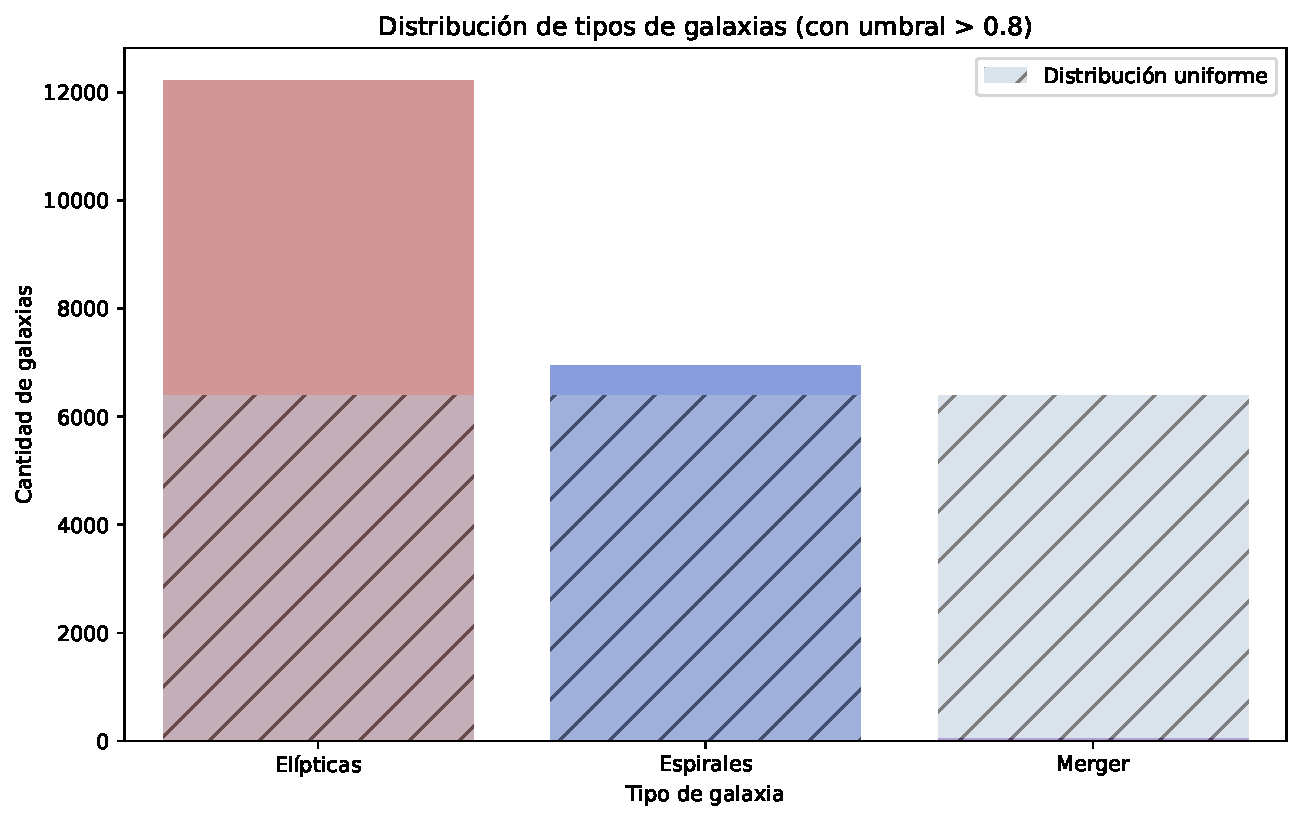
\includegraphics[width=\linewidth]{morfologia.pdf}
\caption{Distribución de frecuencias de tipos morfológicos de galaxias. Las barras representan los valores observados y la línea punteada los valores esperados bajo una distribución uniforme.}
\label{fig:morf}
\end{figure}

SDSS define un tercer tipo de magnitud que, aunque no se utilizó directamente en este trabajo, fundamenta el parámetro \textit{fracDeV}: las \textit{Composite Model Magnitudes} o magnitudes modelo compuestas, definidas como combinación lineal de perfiles de De Vaucouleurs (galaxias elípticas) y exponencial (galaxias espirales):
\[F_{\text{composite}} = \text{fracDeV} \cdot F_{\text{deV}} + (1 - \text{fracDeV}) \cdot F_{\text{exp}}\]

El parámetro \textit{fracDeV} cuantifica cuánto se asemeja el perfil de brillo al perfil de De Vaucouleurs. Valores $\text{fracDeV} \leq 0.2$ indican predominio del disco, mientras que $\text{fracDeV} \geq 0.8$ sugieren predominio del bulbo. Sin embargo, al comparar este parámetro con las clasificaciones de Galaxy Zoo, no se encontró una correlación significativa, indicando que no son intercambiables.

\subsection{Análisis de Magnitudes}

Se trabajó con magnitudes en los filtros $u$, $g$ y $r$, con especial énfasis en el filtro $r$, que SDSS utiliza como referencia para definir propiedades fundamentales como tamaño y parámetro de concentración.

Para ilustrar el método de mínimos cuadrados descrito en la sección 1.1.3, se realizaron ajustes lineales para una submuestra del $10\%$ de la muestra total (por limitaciones computacionales) y para las submuestras de galaxias elípticas y espirales. Los resultados se muestran en la Figura \ref{fig:lineal}.

\begin{figure*}[ht]
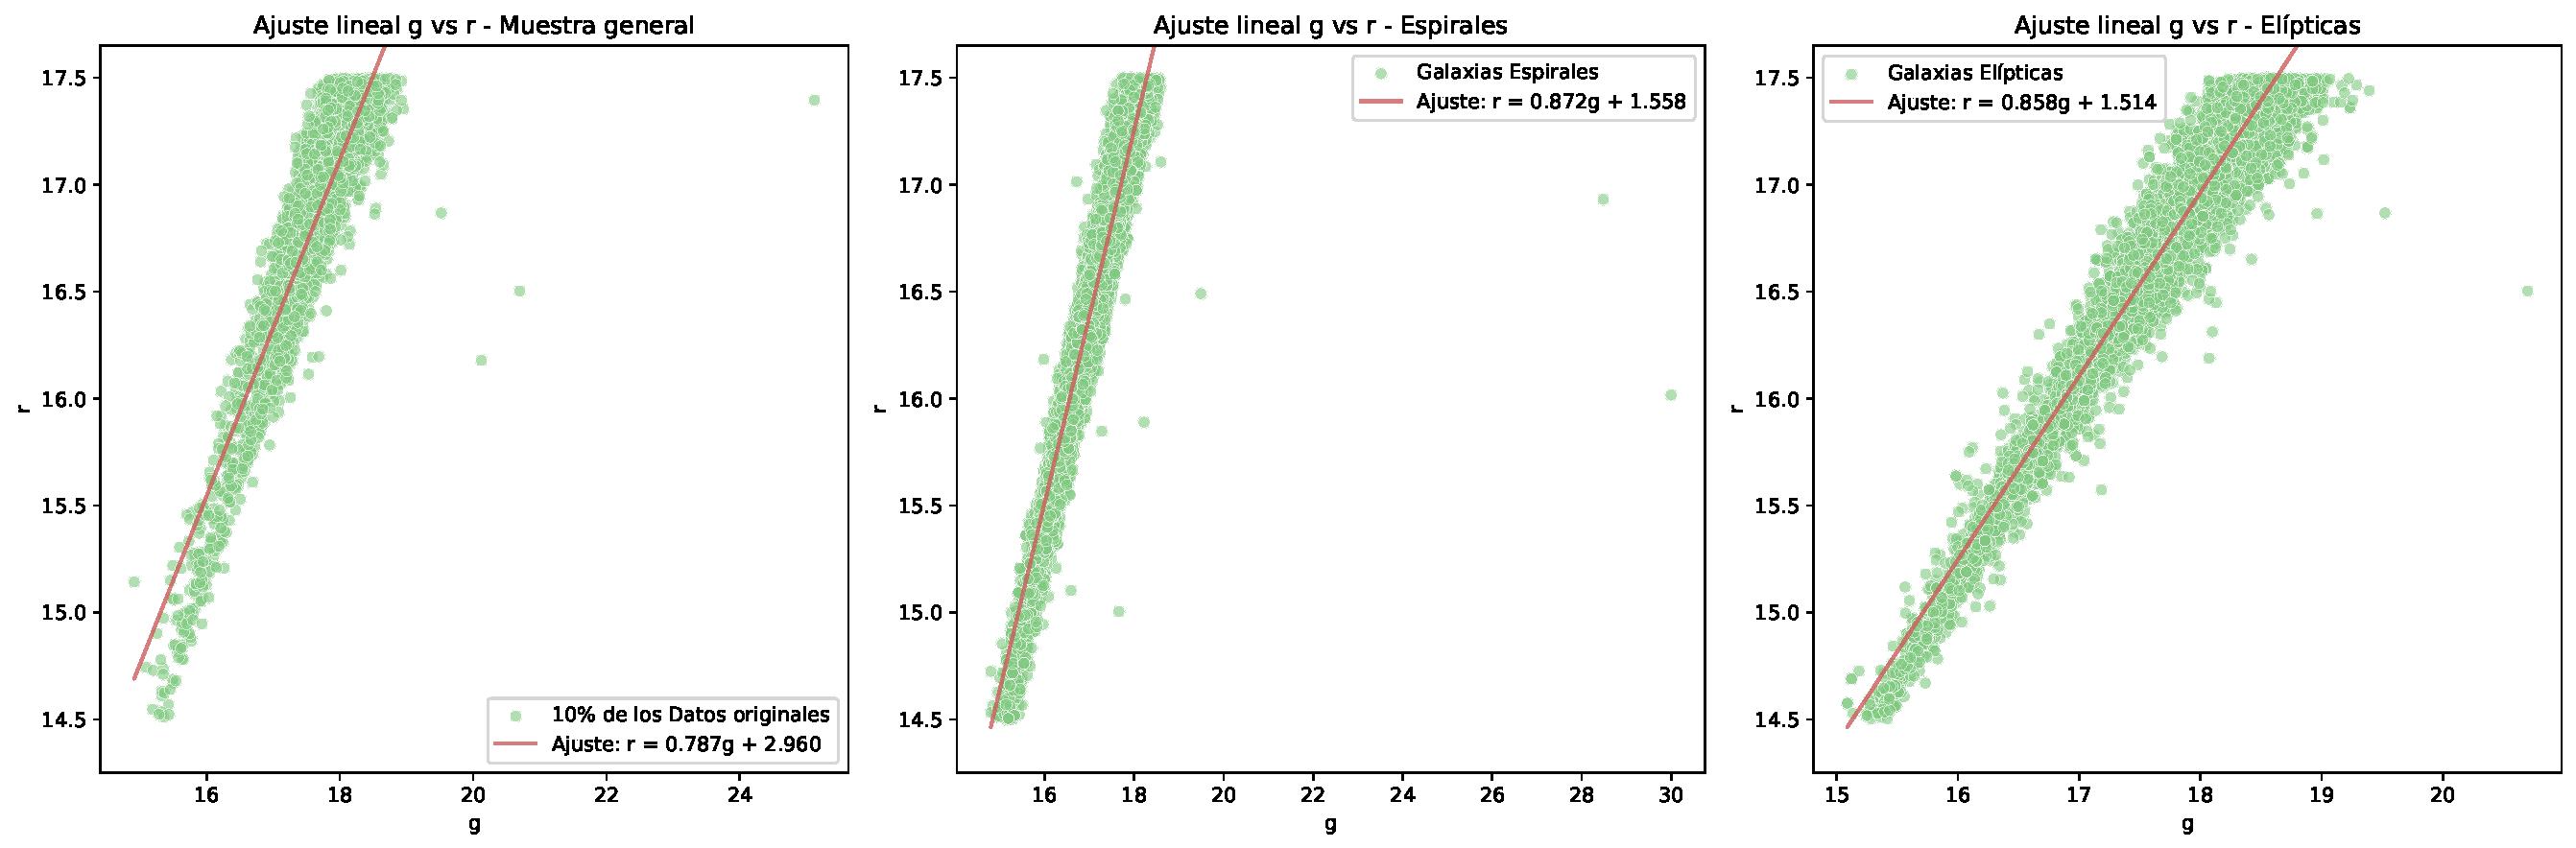
\includegraphics[width=\linewidth]{ajustes_lineales_comparacion.pdf}
\caption{Ajustes lineales $g$ vs $r$ para tres submuestras distintas: muestra completa (izquierda), galaxias elípticas (centro) y galaxias espirales (derecha).}
\label{fig:lineal}
\end{figure*}

\subsubsection{Magnitud Absoluta}

Debido a las grandes distancias involucradas, los efectos cosmológicos deben considerarse al calcular la magnitud absoluta. Se utilizó una aproximación a la distancia luminosa, calculando la magnitud absoluta como:
\begin{equation}
M_r= r - 25 - 5 \log\left(\frac{c \cdot z}{H_0}\right)
\end{equation}
donde $c = 30000$ km s$^{-1}$ es la velocidad de la luz, $H_0 = 75$ km s$^{-1}$ Mpc$^{-1}$ es la constante de Hubble y $z$ es el redshift de cada galaxia.

La Figura \ref{fig:mabs} muestra la relación resultante entre magnitud absoluta y redshift. Los puntos aparecen delimitados por una curva logarítmica (Figura \ref{fig:mabs_log}), efecto atribuible a la extinción por redshift: a mayor redshift, mayor enrojecimiento y menor flujo recibido, haciendo que las galaxias más débiles se vuelvan indetectables.

\begin{figure}[t]
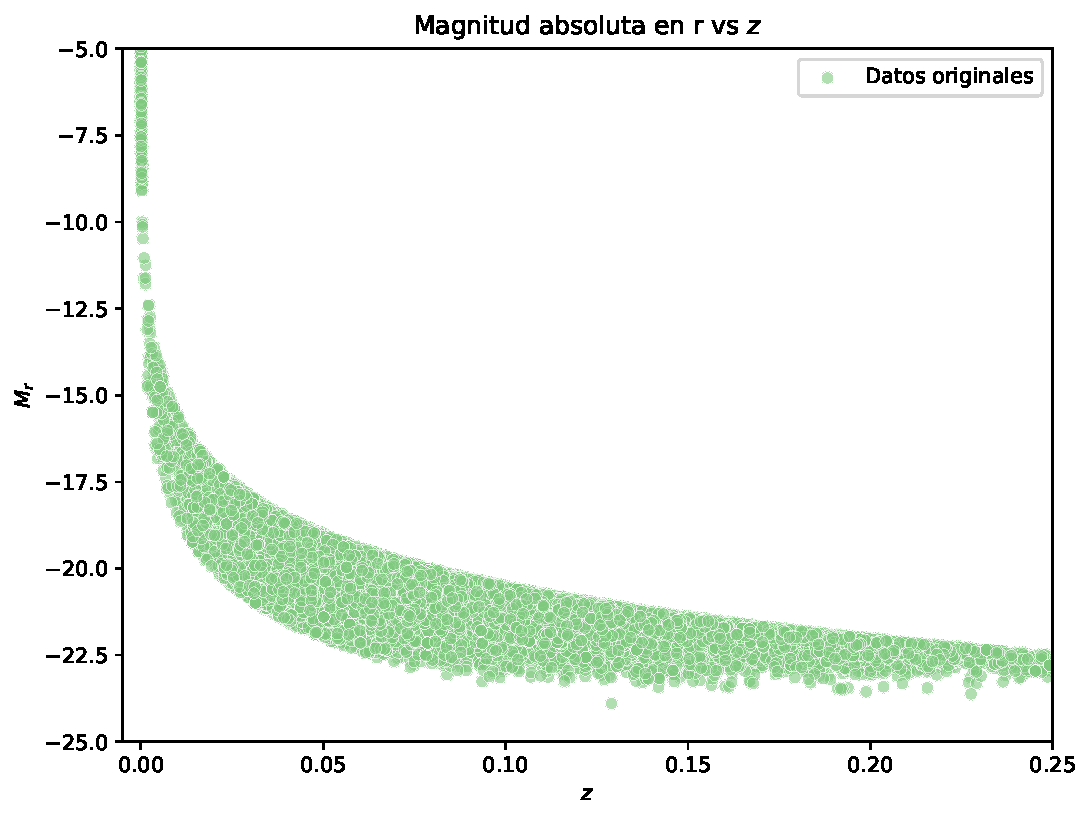
\includegraphics[width=\linewidth]{mabs.pdf}
\caption{Magnitud absoluta en el filtro $r$ vs corrimiento al rojo $z$.}
\label{fig:mabs}
\end{figure}

\begin{figure}[t]
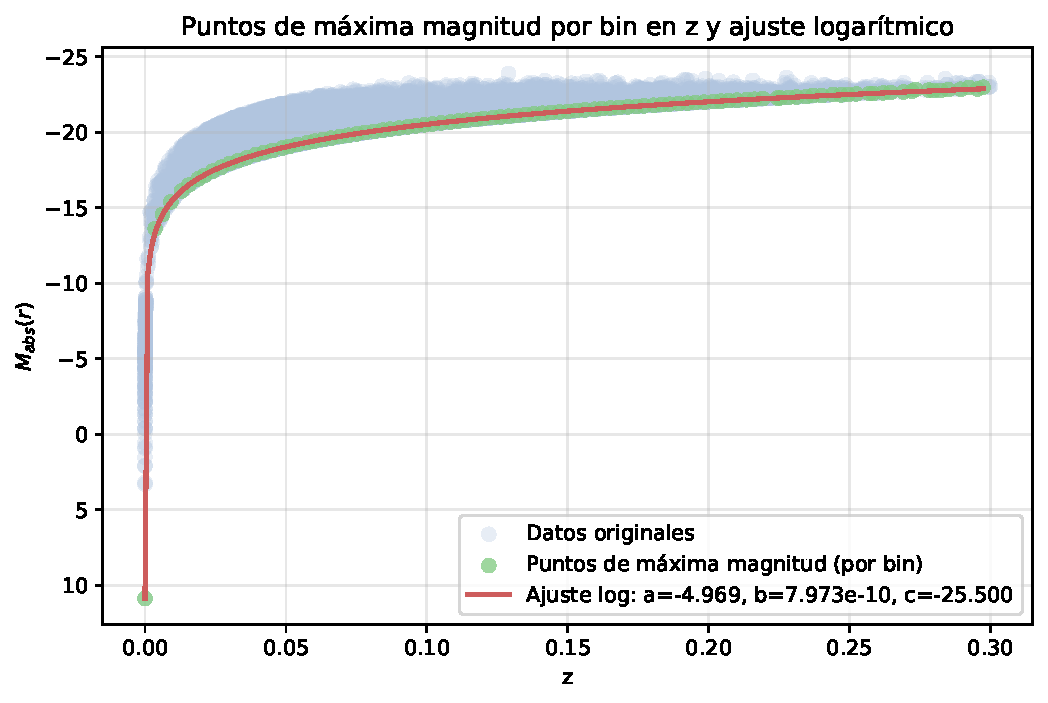
\includegraphics[width=\linewidth]{mabs_vs_z_ajuste_log_max.pdf}
\caption{Magnitud absoluta en el filtro $r$ vs corrimiento al rojo $z$. La línea representa el ajuste logarítmico a la envolvente superior de los puntos.}
\label{fig:mabs_log}
\end{figure}

\subsection{Análisis de Color}

Siguiendo a \citet{2004Bimodalidad}, se sabe que las distribuciones de color en muestras de galaxias presentan bimodalidad, permitiendo ajustar una doble gaussiana que separa las galaxias en rojas ($u-r$ alto) y azules ($u-r$ bajo). La Figura \ref{fig:ur} muestra este análisis para nuestra muestra.

\begin{figure}[t]
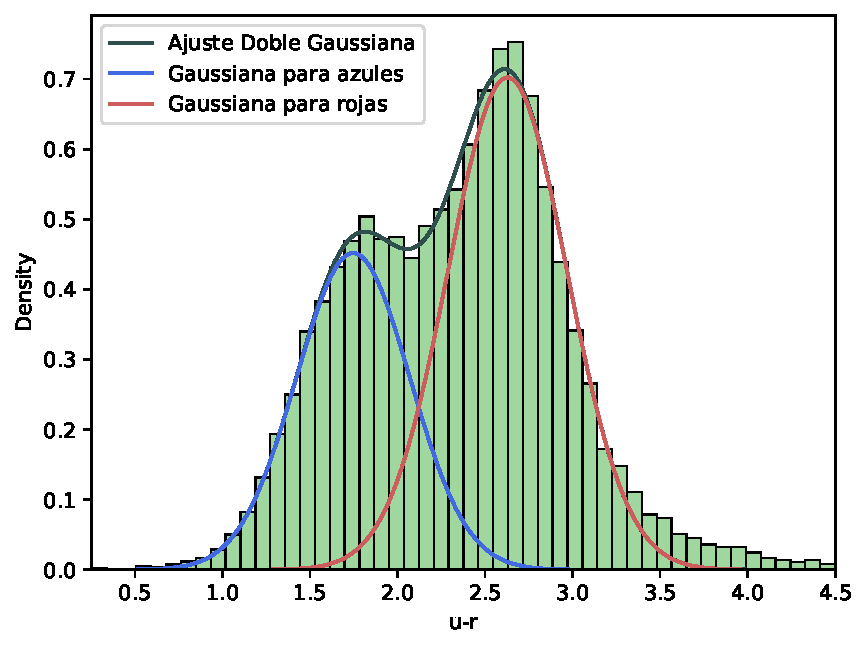
\includegraphics[width=\linewidth]{ur.pdf}
\caption{Distribución del color $u-r$ para las galaxias seleccionadas. El ajuste de doble gaussiana se muestra en línea continua, con cada componente gaussiana representada por líneas punteadas.}
\label{fig:ur}
\end{figure}

Se utilizó la prueba de chi-cuadrado implementada en la librería \textit{SciPy} \citep{SciPy} para verificar la adecuación del modelo de doble gaussiana.

Este análisis se repitió para otros colores ($g-r$ y $u-g$), eligiendo inicialmente $u-r$ por utilizar filtros más separados espectralmente y presentar mayor diferenciación entre los picos (Figura \ref{fig:colores}).

\begin{figure}[t]
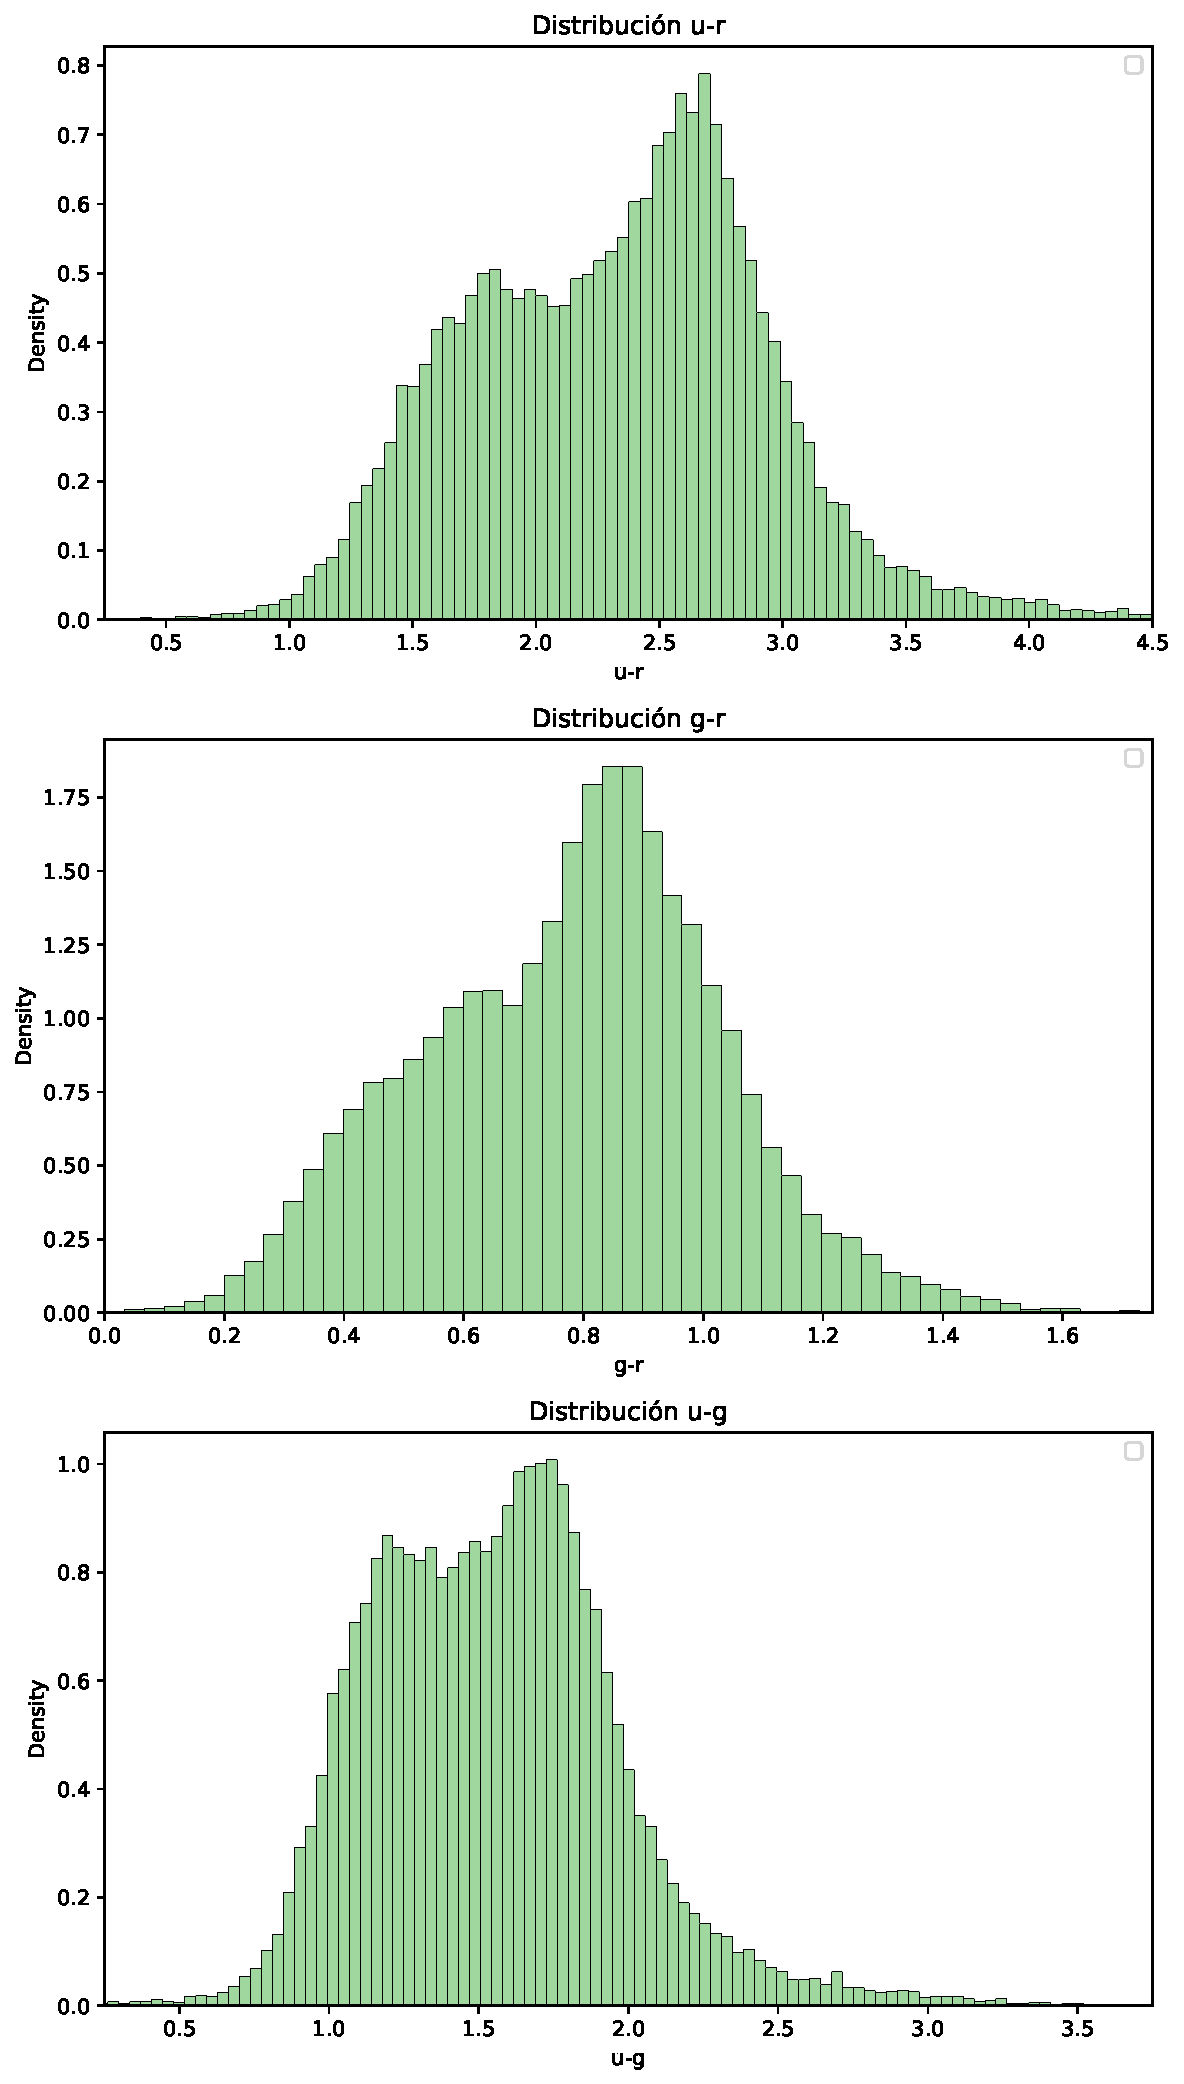
\includegraphics[width=\linewidth]{rojas_azules_vertical.pdf}
\caption{Distribuciones de color para $u-r$, $g-r$ y $u-g$ en la muestra completa.}
\label{fig:colores}
\end{figure}

Al realizar el mismo análisis separando por morfología (Figura \ref{fig:color_forma}), se observa que las distribuciones individuales pierden la bimodalidad presente en la muestra completa. Además, en todos los casos, las galaxias espirales son sistemáticamente más azules que las elípticas. Las pruebas de chi-cuadrado confirmaron que las distribuciones de color difieren significativamente entre tipos morfológicos, sugiriendo una relación intrínseca entre color y morfología.

\begin{figure}[t]
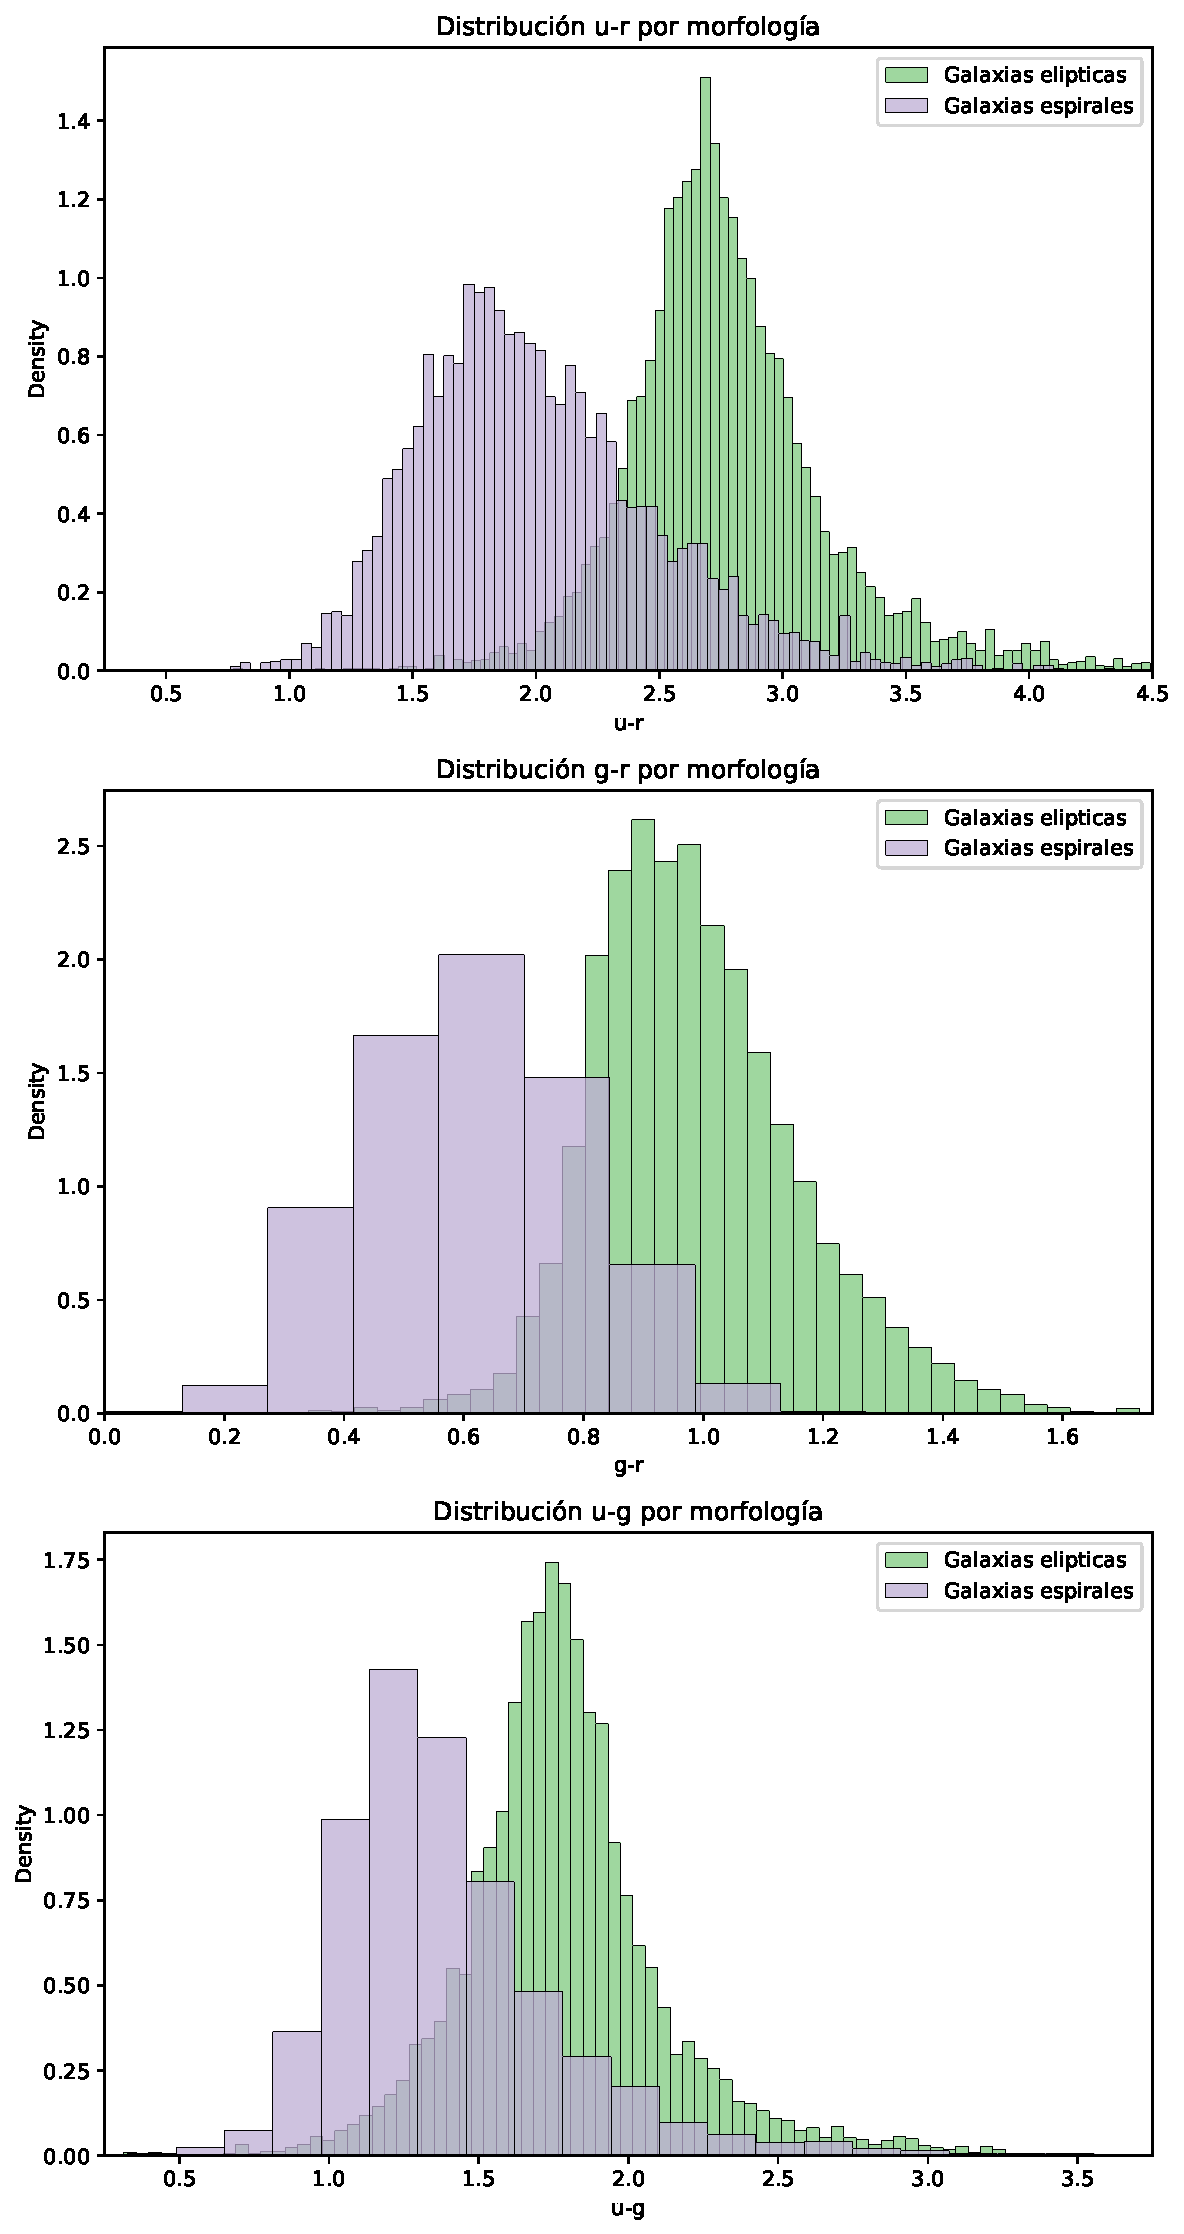
\includegraphics[width=\linewidth]{colores_morfologia_vertical.pdf}
\caption{Distribuciones de color $u-r$, $g-r$ y $u-g$ para galaxias espirales (azul) y elípticas (rojo).}
\label{fig:color_forma}
\end{figure}

\section{Conclusiones}

Este trabajo demuestra la potencia del análisis estadístico y el modelado de datos en astronomía extragaláctica. A través del estudio de una muestra de 50,000 galaxias del SDSS DR19, se han obtenido varios resultados significativos:

\textbf{1. Relación entre morfología y color:} Se confirmó la conocida correlación entre tipo morfológico y propiedades fotométricas, con galaxias elípticas mostrando sistemáticamente colores más rojos ($u-r$ alto) en comparación con las espirales. La pérdida de bimodalidad en las distribuciones de color cuando se separa por morfología sugiere que esta bimodalidad emerge precisamente de la mezcla de poblaciones con diferentes propiedades físicas.

\textbf{2. Efectos observacionales:} Se identificó el efecto de selección debido al redshift, donde las galaxias más débiles se vuelven indetectables a altos redshifts, resultando en una relación característica entre magnitud absoluta y corrimiento al rojo.

\textbf{3. Métodos estadísticos:} Se implementaron exitosamente métodos bayesianos para el ajuste de modelos, particularmente el método de mínimos cuadrados para relaciones lineales y ajustes de doble gaussiana para distribuciones bimodales de color.

\textbf{4. Clasificación morfológica:} Se constató que los parámetros estructurales como \textit{fracDeV} y las clasificaciones visuales de Galaxy Zoo proporcionan información complementaria pero no intercambiable sobre la morfología galáctica.

Estos resultados subrayan la importancia de los enfoques estadísticos para extraer información física robusta de grandes volúmenes de datos astronómicos. Futuros trabajos podrían expandir este análisis incorporando parámetros espectroscópicos, estudiando la evolución temporal de estas relaciones, o aplicando técnicas de machine learning para clasificación y regresión.

\bibliographystyle{plainnat}
\bibliography{bibliografia}

\end{document}